% (c) 2026 Stephanie Märklin, OST Ostschweizer Fachhochschule
%
% !TEX root = ../../buch.tex
% !TEX encoding = UTF-8
%
% Rolle im Paper: Beleg
%
\section{Rechenbeispiel und Vergleich realer Flugzeuge
\label{aircraft:section:6-rechenbeispiel}}
\kopfrechts{Rechenbeispiel}
In diesem Abschnitt wenden wir die Rechnung auf zwei reale Flugzeuge an, ein
einmotoriges Propellerflugzeug und einen Business Jet.
Für beide setzen wir die Derivative aus der Literatur ein und berechnen
Eigenwerte und Eigenvektoren.
Nach Abschnitt~\ref{aircraft:section:5-interpretation} lassen sich
Stabilität und Abklingzeit an den Eigenwerten ablesen.
Der Vergleich zeigt, wie sich zwei Konstruktionen in ihren Eigenwerten
unterscheiden, und damit in ihrer Stabilität.

\subsection{Das Propellerflugzeug
\label{aircraft:section:6-propellerflugzeug}}
Wir betrachten ein einmotoriges Propellerflugzeug im Horizontalflug.
Die Derivative für diesen Flugzustand stammen aus
Nelson~\cite[Tabelle 5.2 und Anhang B]{aircraft:nelson}.
Die Systemmatrix lautet damit
\begin{equation}
    A
    =
    \begin{pmatrix}
        -0.254 &  0     & -1.0   & 0.182 \\
        -16.02  & -8.40  &  2.19  & 0     \\
        4.488 & -0.350 & -0.760 & 0     \\
        0     &  1     &  0     & 0
    \end{pmatrix}.
    \label{aircraft:eqn:systemmatrix-ga}
\end{equation}
Die Nullstellen der charakteristischen Gleichung berechnen wir numerisch mit
MATLAB.
Das ergibt die vier Eigenwerte und ihre Halbwertszeiten nach
Gleichung~\eqref{aircraft:eqn:halbwertszeit},
\begin{align}
    \lambda_1     &= -8.433,              & t_{1/2} &= 0.08\,\text{s},
    \notag \\
    \lambda_2     &= -0.00891,            & t_{1/2} &= 78\,\text{s},
    \notag \\
    \lambda_{3,4} &= -0.486 \pm 2.334\,i, & t_{1/2} &= 1.4\,\text{s},
    \quad T = 2.7\,\text{s}.
    \label{aircraft:eqn:eigenwerte-ga}
\end{align}
Sie stimmen bis auf Rundungsunterschiede in den Derivativen mit den von
Nelson~\cite[Beispiel 5.3]{aircraft:nelson} angegebenen Werten überein.
Zwei Eigenwerte sind reell, zwei bilden ein komplexes Paar.
Nach Abschnitt~\ref{aircraft:section:5-eigenvektoren} besteht die
Seitenbewegung dieses Flugzeugs also aus zwei Eigenbewegungen ohne Schwingung
und einer Schwingung.

Welche Bewegungsform zu welchem Eigenwert gehört, lesen wir nach
Abschnitt~\ref{aircraft:section:5-eigenvektoren} an den Eigenvektoren ab.
Ein Eigenvektor ist nach Abschnitt~\ref{aircraft:section:4-eigenwerte} nur bis
auf einen Faktor bestimmt.
Wir teilen deshalb jeden Eigenvektor durch seine betragsgrösste Komponente,
so dass diese den Wert $1$ hat und die übrigen als Anteile davon erscheinen.
Die Tabelle~\ref{aircraft:table:eigenvektoren-ga} enthält die Beträge dieser
Komponenten.
Beim Eigenwert $\lambda_1$ sind nur die Rollrate und der Rollwinkel
nennenswert, beides Grössen der Längsachse, diese Eigenbewegung ist die
Rollbewegung.
Beim Eigenwert $\lambda_2$ dominiert der Rollwinkel, begleitet von einer
kleinen Gierrate, das ist das langsame Kippen mit Kursänderung der
Spiralbewegung.
Beim Paar $\lambda_{3,4}$ sind alle vier Komponenten von derselben
Grössenordnung.
Damit ist diese Eigenbewegung gekoppelt im Sinne von
Abschnitt~\ref{aircraft:section:system}, das ist die Dutch Roll.
Die drei Eigenbewegungen sind genau die drei Bewegungsformen aus
Abschnitt~\ref{aircraft:section:1-grundbegriffe}.

Mit der Zuordnung lassen sich die Halbwertszeiten aus
Gleichung~\eqref{aircraft:eqn:eigenwerte-ga} deuten.
Die Rollbewegung ist nach einer Zehntelsekunde auf die Hälfte abgeklungen.
Die Spiralbewegung braucht dafür über eine Minute und verläuft nach
Nelson~\cite[Abschnitt 5.1]{aircraft:nelson} so allmählich, dass der Pilot
sie nicht bewusst wahrnimmt.
Die Dutch Roll ist nach etwa einer halben Periode auf die Hälfte abgeklungen.
Alle vier Realteile sind negativ.
Die Seitenbewegung dieses Flugzeugs ist nach
Abschnitt~\ref{aircraft:section:5-interpretation} also stabil.
Damit ist die Frage aus Abschnitt~\ref{aircraft:section:1-grundbegriffe}
für dieses Flugzeug beantwortet.
Es kehrt in die Ruhelage zurück, und die Halbwertszeiten geben an, wie
schnell.

\begin{table}
    \centering
    \begin{tabular}{llrrrr}
        \hline
        Eigenwert & Bewegungsform & $|\beta|$ & $|p|$ & $|r|$ & $|\varphi|$ \\
        \hline
        $\lambda_1 = -8.433$                  & Rollbewegung
        & $0.008$ & $1.000$ & $0.041$ & $0.119$ \\
        $\lambda_2 = -0.00891$                & Spiralbewegung
        & $0.029$ & $0.009$ & $0.175$ & $1.000$ \\
        $\lambda_{3,4} = -0.486 \pm 2.334\,i$ & Dutch Roll
        & $0.454$ & $0.890$ & $1.000$ & $0.374$ \\
        \hline
    \end{tabular}
    \caption{Beträge der Eigenvektorkomponenten des Propellerflugzeugs,
        normiert auf die grösste Komponente, und die daraus abgelesene
        Bewegungsform.
        \label{aircraft:table:eigenvektoren-ga}}
\end{table}

\subsection{Der Business Jet
\label{aircraft:section:6-businessjet}}
Für den Business Jet gibt
Stengel~\cite[Lecture 20, Supplemental Material]{aircraft:stengel} die
Systemmatrix an, mit den Zustandsgrössen in der Reihenfolge $r$, $\beta$,
$p$, $\varphi$.
In der Reihenfolge von Gleichung~\eqref{aircraft:eqn:zustandsvektor}
umgeordnet lautet sie
\begin{equation}
    A
    =
    \begin{pmatrix}
        -0.1567 &  0      & -1      & 0.0958 \\
        -2.408  & -1.1616 &  0.2501 & 0      \\
        1.9011 &  0.0566 & -0.1079 & 0      \\
        0      &  1      &  0      & 0
    \end{pmatrix}.
    \label{aircraft:eqn:systemmatrix-bizjet}
\end{equation}
Dieselbe Rechnung wie beim Propellerflugzeug ergibt
\begin{align}
    \lambda_1     &= -1.203,              & t_{1/2} &= 0.6\,\text{s},
    \notag \\
    \lambda_2     &= +0.00883,            & t_{1/2} &= -78\,\text{s},
    \notag \\
    \lambda_{3,4} &= -0.116 \pm 1.390\,i, & t_{1/2} &= 6.0\,\text{s},
    \quad T = 4.5\,\text{s}.
    \label{aircraft:eqn:eigenwerte-bizjet}
\end{align}

Auch hier sind zwei Eigenwerte reell und zwei bilden ein Paar, und die
Eigenvektoren in Tabelle~\ref{aircraft:table:eigenvektoren-bizjet} zeigen
dieselbe Zuordnung wie beim Propellerflugzeug.
Bei der Rollbewegung ist der Rollwinkel grösser als beim Propellerflugzeug,
weil die Drehung langsamer abklingt und sich dabei mehr Rollwinkel ansammelt.

Die Rollbewegung klingt langsamer ab als beim Propellerflugzeug, aber immer
noch rasch.
Der Eigenwert der Spiralbewegung ist positiv, die Seitenbewegung dieses
Flugzeugs ist also instabil.
Die negative Halbwertszeit ist nach
Abschnitt~\ref{aircraft:section:5-interpretation} eine Verdoppelungszeit
von $78$\,s.
Eine Störung braucht über eine Minute, um sich zu verdoppeln.
Nelson~\cite[Tabelle 5.4]{aircraft:nelson} verlangt für gute
Flugeigenschaften eine Verdoppelungszeit von mindestens $20$\,s, ein
Pilot korrigiert diese Spiralbewegung also nebenbei.
Damit ist die Aussage aus Abschnitt~\ref{aircraft:section:1-grundbegriffe}
bestätigt, dass die Spiralbewegung leicht korrigierbar ist.
Die Dutch Roll ist stabil, braucht aber mehr als eine Periode, bis sie auf
die Hälfte abgeklungen ist, beim Propellerflugzeug reicht dafür eine halbe
Periode.

\begin{table}
    \centering
    \begin{tabular}{llrrrr}
        \hline
        Eigenwert & Bewegungsform & $|\beta|$ & $|p|$ & $|r|$ & $|\varphi|$ \\
        \hline
        $\lambda_1 = -1.203$                  & Rollbewegung   & $0.010$
        & $1.000$ & $0.069$ & $0.831$ \\
        $\lambda_2 = +0.00883$                & Spiralbewegung & $0.006$
        & $0.009$ & $0.095$ & $1.000$ \\
        $\lambda_{3,4} = -0.116 \pm 1.390\,i$ & Dutch Roll     & $0.718$
        & $1.000$ & $0.954$ & $0.717$ \\
        \hline
    \end{tabular}
    \caption{Beträge der Eigenvektorkomponenten des Business Jets,
        normiert auf die grösste Komponente, und die daraus abgelesene
        Bewegungsform.
        \label{aircraft:table:eigenvektoren-bizjet}}
\end{table}

\subsection{Vergleich
\label{aircraft:section:6-vergleich}}
Die Tabelle~\ref{aircraft:table:vergleich} stellt Dämpfung, Frequenz,
Periode und Halbwertszeit der drei Bewegungsformen beider Flugzeuge
gegenüber.
Die Abbildung~\ref{aircraft:fig:komplexe-ebene} zeigt die Eigenwerte in der
komplexen Ebene.
Der Abstand eines Eigenwerts von der imaginären Achse ist seine Dämpfung,
sein Abstand von der reellen Achse seine Frequenz.
Beide Flugzeuge haben dieselben drei Bewegungsformen, die Eigenwerte liegen
aber an verschiedenen Stellen.
Die Rollbewegung des Propellerflugzeugs liegt weit links, die des Business
Jets nahe bei den anderen Eigenwerten.
Die beiden Spiralbewegungen liegen fast am selben Ort, aber auf
verschiedenen Seiten der imaginären Achse, und das entscheidet über die
Stabilität.
Die Dutch Roll des Business Jets liegt näher bei der imaginären Achse als
die des Propellerflugzeugs, sie ist schwächer gedämpft.
Die Stabilität und die Abklingzeiten beider Flugzeuge lassen sich damit
vollständig aus der Lage der Eigenwerte ablesen.

\begin{table}
    \centering
    \begin{tabular}{llrrrr}
        \hline
        Flugzeug & Bewegungsform
        & $\sigma$ & $\omega$ & $T$ [s] & $t_{1/2}$ [s] \\
        \hline
        Propellerflugzeug & Rollbewegung
        & $-8.433$           & --      & --    & $0.08$ \\
        & Spiralbewegung
        & $-0.00891$         & --      & --    & $78$   \\
        & Dutch Roll
        & $-0.486$           & $2.334$ & $2.7$ & $1.4$  \\
        \hline
        Business Jet      & Rollbewegung
        & $-1.203$           & --      & --    & $0.6$  \\
        & Spiralbewegung
        & $+0.00883$         & --      & --    & $-78$  \\
        & Dutch Roll
        & $-0.116$           & $1.390$ & $4.5$ & $6.0$  \\
        \hline
    \end{tabular}
    \caption{Dämpfung, Frequenz, Periode und Halbwertszeit der drei
    Bewegungsformen beider Flugzeuge.
    Die negative Halbwertszeit der Spiralbewegung des Business Jets ist eine
    Verdoppelungszeit.
    \label{aircraft:table:vergleich}}
\end{table}

\begin{figure}
    \centering
    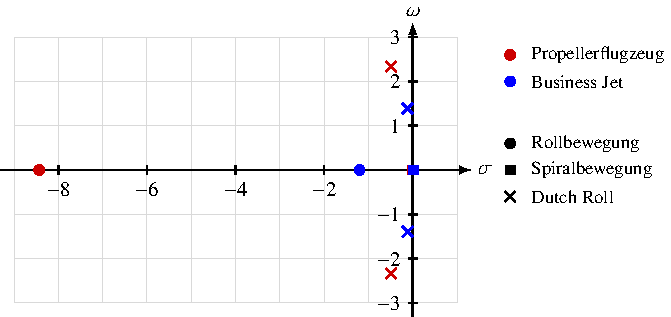
\includegraphics{papers/aircraft/images/komplexe-ebene.pdf}
    \caption{Eigenwerte des Propellerflugzeugs und des Business Jets in
    der komplexen Ebene.
    Die Farbe unterscheidet die Flugzeuge, der Marker die Bewegungsform.
    Die Eigenwerte der beiden Spiralbewegungen liegen bei $-0.009$ und
        $+0.009$ und sind in dieser Skala nicht zu unterscheiden.
        \label{aircraft:fig:komplexe-ebene}}
\end{figure}


